\subsubsection{Accuracy and execution results}
No conditional-bound violation occurs in the 1,152 independent observable comparisons. The linear predictor underestimates the observed change by more than $10^{-12}$ in 373 comparisons; these are prediction underestimates, not acceptance-budget violations. Maximum disagreement between occurrence shifts and the independent finite differences is $3.75\times10^{-11}$. In the analytic single-qubit step sweep at $\theta=0.37$, central differences have derivative error $6.03\times10^{-10}$ at step $10^{-4}$, but $0.362$ at step $10^{-16}$, where subtraction returns zero. Parameter shift has error $5.55\times10^{-17}$ on this fixture. This illustrates cancellation, not a universal optimal finite-difference step.

Uniform rounding violates the $10^{-6}$ budget on all nine timing fixtures and the $10^{-4}$ budget on four. Bounded selection has no observed violations and changes zero and five fixtures, respectively; at $0.01$, it changes all nine. Gradient-only acceptance has no budget violation in this small weak-bridge sweep, but fails the separate stationary-point counterexample. These controls support including a remainder term without claiming that every small-gradient approximation fails. Across 1,134 warm collections, 162 first collections and 162 resource probes, the maximum native disagreement with the corresponding original or modified NumPy reference is $1.24\times10^{-15}$; approximation bias is reported separately.

On the two-block 16-qubit fixtures, approximation reduces the largest state from 16 to eight qubits ($256\times$ payload reduction). Serial warm execution falls from 63.21--67.36\,ms to 1.17--1.65\,ms across sessions and seeds, giving $40.56\times$--$53.88\times$. However, profiling costs 133.05--165.46\,ms. The eight-collection lifetime speedup is consequently $2.89\times$--$3.57\times$, with observed sustained break-even in two to three collections. Maximum approximation bias is $1.14\times10^{-5}$, below a maximum conditional bound of $1.62\times10^{-5}$. Two workers lower profiling to 87.83--103.89\,ms, but the small approximate tasks and process setup limit lifetime speedup to $2.27\times$--$2.57\times$.

Three-block 15-qubit fixtures reduce maximum width to five ($1024\times$ payload reduction), with maximum observed bias $2.06\times10^{-4}$. Serial warm speedups of $30.95\times$--$35.46\times$ become $1.31\times$--$1.55\times$ after all charges. Four-worker lifetime results span $0.99\times$--$1.10\times$. The eight-qubit cases regress over eight collections at every worker count. The connected 16-qubit control retains width 16 and has lifetime ratios of $0.77\times$--$0.85\times$ despite admissible angle changes. Thus angle approximation needs both exploitable structure and enough reuse to repay analysis.

Figure~\ref{fig:sensitivity} presents error control and charged execution; Table~\ref{tab:sensitivity-results} retains all fixture/worker families in the Appendix. Payload reductions do not imply comparable RSS reductions: in the serial 16-qubit weak-bridge probes, both policies retain approximately 51--52\,MiB sampled RSS. Four workers raise the sampled parent-plus-pool sum to approximately 220--223\,MiB. Allocator retention and shared-page accounting limit interpretation. RQ4 has positive evidence on constructed weak bridges, with explicit negative controls; it does not establish general variational-circuit acceleration or automatic selection of approximation and worker policies.

\begin{figure*}[t]
\centering
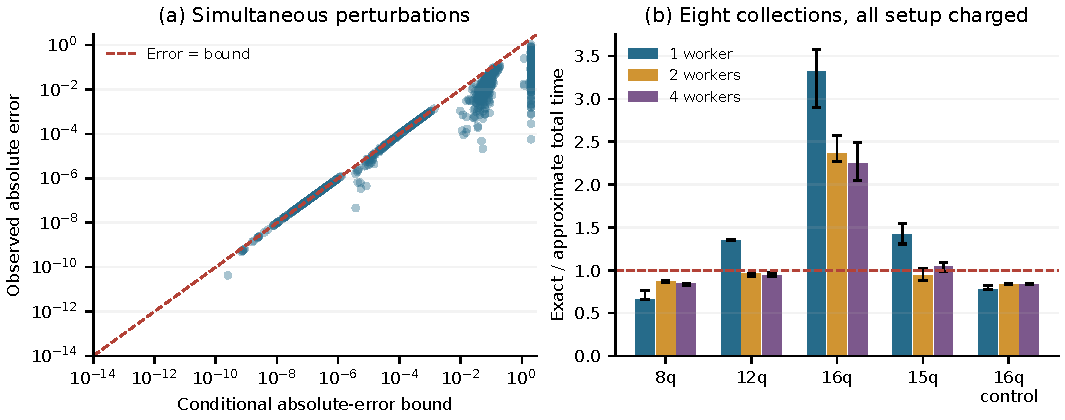
\includegraphics[width=0.98\textwidth]{figures/sensitivity_tradeoff.pdf}
\caption{Observable-sensitivity validation. (a) Actual errors versus conditional bounds for simultaneous perturbations; zero points are omitted on logarithmic axes. (b) Median eight-collection lifetime ratios, with whiskers spanning session/seed configurations rather than confidence intervals. Each ratio compares exact and approximate execution at the same worker count. Profiling, search and worker setup/shutdown are charged.}
\label{fig:sensitivity}
\end{figure*}
